\begin{wrapfigure}{r}{5cm}
%	\centering
%\begin{center}
	\setbox0\hbox{
		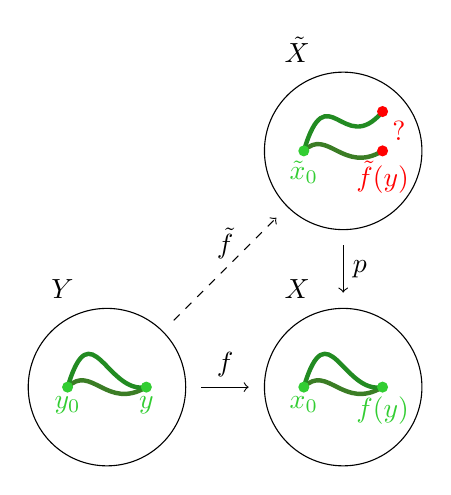
\begin{tikzpicture}[yscale=1]
		% Räume
		\draw (-3,0) 
			circle (1cm) 
			node[above left,xshift=-0.3cm,yshift=1cm] {$Y$};
		
		\draw (0,0) 
			circle (1cm) 
			node[above left,xshift=-0.3cm, yshift=1cm]{$X$};
		
		\draw (0,3) 
			circle (1cm) 
			node[above left,xshift=-0.3cm,yshift=1cm]{$\tilde{X}$};	
		%Abbildungen
		\draw[->] (-1.8,0) 
			-- 
			node[above] {$f$} (-1.2,0) ;
		\draw[->] (0,1.8) 
			-- 
		node[right] {$p$} (0,1.2) ;
		\draw[dashed, ->, shorten >= 1.2cm, shorten <= 1.2cm] (-3,0) 
			-- node[above] {$\tilde{f}$} (0,3) ;
		%Wege
		\def\Weg#1#2{
		\begin{scope}[xshift=#1cm,yshift=#2cm]
			\draw[ultra thick, OliveGreen] 
				(0,0) 
				.. controls (0.3,0.3) and (0.5,-0.3) ..
				%to[out=60,in=120] 
				++(1,0);
				\ifnum#2<3
					\draw[ultra thick, ForestGreen] 
					(0,0) 
					.. controls (0.3,1) and (0.5,-0.1) ..
					%to[out=60,in=120] 
					++(1,0);
				\fi	
		\end{scope}
		}
		\Weg{-0.5}{0}
		\Weg{-3.5}{0}
		\Weg{-0.5}{3}
		 %FrageWeg
		 	\begin{scope}[xshift=-0.5cm, yshift=3cm]
				\draw[ultra thick, ForestGreen] 
					(0,0) 
					.. controls (0.3,1) and (0.5,-0.1) ..
					%to[out=60,in=120] 
					++(1,0.5);
			\fill[red] (1,0.5) 
				circle (2pt)
				node[below right] {?}
				node[below] {$\shortparallel$};
			\end{scope}
		%Punkte
		\fill[LimeGreen, xshift=-0.5cm] (-3,0)
			circle (2pt)
			node[below] {$y_0$};
		\fill[LimeGreen, xshift=-0.5cm] (0,0)
			circle (2pt)
			node[below] {$x_0$};
		\fill[LimeGreen, xshift=-0.5cm] (0,3)
			circle (2pt)
			node[below] {$\tilde{x}_0$};
		\fill[LimeGreen, xshift=+0.5cm]
		(-3,0)
			circle (2pt)
			node[below] {$y$};
		\fill[LimeGreen, xshift=+0.5cm]
		(0,0)
			circle (2pt)
			node[below] {$f(y)$};
		\fill[red, xshift=+0.5cm]
		(0,3)
			circle (2pt)
			node[below] {$\tilde{f}(y)$};
	\end{tikzpicture}
	}
	\ht0=140pt
	\box0
%\end{center}
\end{wrapfigure}